\section{Parametrised curves, lengths and arc length}

\begin{ndefi}[Parametrisation]
	Given a curve $C$ in $\mathbb{R}^n$, a \emph{parametrisation} of it is a continuous and invertible function $\mathbf{r}: D \rightarrow \mathbb{R}^n$ for some $D \subseteq \mathbb{R}$ whose image is $C$. Parametrisation is therefore the function mapping a real input into a vector output.
\end{ndefi}

\begin{remark}
  Parametrisation of a curve is not unique, different parametrisations could trace out the same curve.  
\end{remark}

\begin{definition}[Closed and Simple]
  If $\boldsymbol{x}\left(t_1\right)=\boldsymbol{x}\left(t_0\right)$ then the curve is called closed. A curve that does not cross itself is called simple.
\end{definition}

\begin{ndefi}[Differentiable Parametrisation]
	A parametrisation $\boldsymbol{x}(t)$ is differentiable if it has a well-defined tangent vector,
	
	$$
	\frac{d \boldsymbol{x}}{d t}=\lim _{d t \rightarrow 0} \frac{\boldsymbol{x}(t+d t)-\boldsymbol{x}(t)}{d t},
	$$
	
	so-called because its direction points along the curve at each $t$.
\end{ndefi}

\begin{ndefi}[Regular Parametrisation]
	A parametrisation is regular if $\frac{d \boldsymbol{x}}{d t} \neq 0$ everywhere, and a curve is regular if it has at least one regular parametrisation.
\end{ndefi}

\begin{ndefi}[Singular Parametrisation and Cusps]
	
	A parametrisation is singular if $\frac{d \boldsymbol{x}}{d t} = 0$ at at least one point. The singular points of a parametrisation are called susps.
	
\end{ndefi}

\begin{nrem}
	You can construct a singular parametrisation even for a regular curve.
\end{nrem}


\begin{nprop}[Change in Arclength of a curve]
	Let $s$ denote the arclength of a curve $\mathbf{r}(u)$. Then
	
	$$
	\frac{\mathrm{d} s}{\mathrm{~d} u}= \pm\left|\frac{\mathrm{d} \mathbf{r}}{\mathrm{~d} u}\right|= \pm\sqrt{\frac{\mathrm{d} \mathbf{r}}{\mathrm{~d} u} \cdot \frac{\mathrm{d} \mathbf{r}}{\mathrm{~d} u}}=  \pm\left|\mathbf{r}^{\prime}(u)\right|
	$$
	
	with the sign depending on whether it is in the direction of increasing or decreasing arclength.
\end{nprop}

\begin{nrem}[Arclength]
	Using the formula above, the arc length between two points on the curve $\mathbf{r}(u)$, given by $u=u_1$ and $u=u_2$, is
	
	\begin{equation}
		s=\int_{u_1}^{u_2} \sqrt{\frac{d \mathbf{r}}{d u} \cdot \frac{d \mathbf{r}}{d u}} d u 
	\end{equation}
	
\end{nrem}

\begin{nmeth}[Deriving tiny change in Arclength]
	The tiny displacement vector is
	
	$$
	d \mathbf{r}=\mathbf{r}^{\prime}(u) d u
	$$
	
	
	Its magnitude gives the tiny distance travelled:
	
	$$
	d s=|d \mathbf{r}|
	$$
	
	
	Hence
	
	$$
	d s=\left|\mathbf{r}^{\prime}(u) d u\right|
	$$
	
	and since $d u$ is scalar,
	
	$$
	d s=\left|\mathbf{r}^{\prime}(u)\right||d u|
	$$
	
	which becomes
	
	$$
	d s=\left|\mathbf{r}^{\prime}(u)\right| d u
	$$
	
	when moving in the positive parameter direction.
\end{nmeth}

\section{Line Integrals of Scalar Fields}

\begin{ndefi}[Scalar Line Element]
	The scalar line element of $C$ is $\mathrm{d} s$.
\end{ndefi}

\begin{nprop}[Formula for Scalar Line Element]
	$\mathrm{d} s= \pm\left|\mathbf{r}^{\prime}(u)\right| \mathrm{d} u$
\end{nprop}

\begin{ndefi}[Line Integral of a Scalar Field]
	The line integral of a scalar field $f(\boldsymbol{x})$ along a curve $C$ with parametrisation $\boldsymbol{x}(t)$, for $t \in\left[t_0, t_1\right]$, is defined as
	
	$$
	\int_C f \, ds=\int_{t_0}^{t_1} f(\boldsymbol{x}(t))\left|\frac{d \boldsymbol{x}}{d t}\right| d t .
	$$
\end{ndefi}

\begin{nprop}[*Choice of Parametrisation doesn't matter]
	The line integral of a scalar field is independent of the choice of parametrisation.
\end{nprop}

\begin{proof}
  Insert a proof here
\end{proof}

\begin{nrem}
	The arclength formula from before is therefore the line integral of the scalar field $f(\mathbf{x}) = 1$
\end{nrem}

\begin{ndefi}[Rectifiable]
	
	A curve which has finite length is called rectifiable. This is a weaker condition than "regular" (for example, if $\boldsymbol{x}(t)$ is Lipschitz continuous then it is rectifiable).
	
\end{ndefi}


\section{Line Integral of Vector Fields}

\begin{ndefi}[Line Integral of a Vector Field]
	The \emph{line integral} of a smooth vector field $\mathbf{F}(\mathbf{r})$ along a path $C$ parametrised by $\mathbf{r}(u)$ along the direction (orientation) $\mathbf{r}(\alpha) \rightarrow \mathbf{r}(\beta)$ is
	
	$$
	\int_C \mathbf{F}(\mathbf{r}) \cdot \mathrm{d} \mathbf{r}=\int_\alpha^\beta \mathbf{F}(\mathbf{r}(u)) \cdot \mathbf{r}^{\prime}(u) \mathrm{d} u
	$$
	
	
	We say $\mathrm{d} \mathbf{r}=\mathbf{r}^{\prime}(u) \mathrm{d} u$ is the line element on $C$. Note that the upper and lower limits of the integral are the end point and start point respectively, and $\beta$ is not necessarily larger than $\alpha$.
\end{ndefi}

\begin{nex}[Showing Line Integral depends on Curve]
	
	
	Take $\mathbf{F}(\mathbf{r})=\left(x e^y, z^2, x y\right)$ and we want to find the line integral from $\mathbf{a}=(0,0,0)$ to $\mathbf{b}=(1,1,1)$. 
	
	\begin{figure}[H]
		
		\centering
		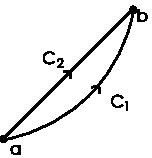
\includegraphics[width=0.3\textwidth]{figures/lineintegral.pdf}
		\caption{Two curves between $a$ and $b$ }
	\end{figure}
	
	
	We first integrate along the curve $C_1: \mathbf{r}(u)=\left(u, u^2, u^3\right)$. Then $\mathbf{r}^{\prime}(u)= \left(1,2 u, 3 u^2\right)$, and $\mathbf{F}(\mathbf{r}(u))=\left(u e^{u^2}, u^6, u^3\right)$. So
	
	$$
	\begin{aligned}
		\int_{C_1} \mathbf{F} \cdot \mathrm{~d} \mathbf{r} & =\int_0^1 \mathbf{F} \cdot \mathbf{r}^{\prime}(u) \mathrm{d} u \\
		& =\int_0^1 u e^{u^2}+2 u^7+3 u^5 \mathrm{~d} u \\
		& =\frac{e}{2}-\frac{1}{2}+\frac{1}{4}+\frac{1}{2} \\
		& =\frac{e}{2}+\frac{1}{4}
	\end{aligned}
	$$
	
	Now we try to integrate along another curve $C_2: \mathbf{r}(t)=(t, t, t)$. So $\mathbf{r}^{\prime}(t)= (1,1,1)$.
	
	$$
	\begin{aligned}
		\int_{C_2} \mathbf{F} \cdot \mathrm{~d} \mathbf{r} & =\int \mathbf{F} \cdot \mathbf{r}^{\prime}(t) \mathrm{d} t \\
		& =\int_0^1 t e^t+2 t^2 \mathrm{~d} t \\
		& =\frac{5}{3}
	\end{aligned}
	$$
	
	
	We see that the line integral depends on the curve $C$ in general, not just $\mathbf{a}, \mathbf{b}$.
\end{nex}

\begin{ndefi}[Unit Tangent]
	The unit tangent vector of a parametrisation is
	
	$$
	\hat{\boldsymbol{t}}=\frac{\frac{d \boldsymbol{x}}{d t}}{\left|\frac{d \boldsymbol{x}}{d t}\right|}
	$$
	
	
	This only depends on the direction of the parametrisation, not the "speed".
\end{ndefi}

\begin{ndefi}[Oriented Curve]
	An oriented curve is a curve together with a specified (consistent) choice of $\hat{\boldsymbol{t}}$. We indicate this by adding an arrow to the curve.
\end{ndefi}

\begin{ndefi}[Line Integral along an Oriented Curve]
	The line integral of a vector field $\boldsymbol{f}(\boldsymbol{x})$ along an oriented curve $C$ with parametrisation $\boldsymbol{x}(t)$, for $t \in\left[t_0, t_1\right]$, is defined as the scalar line integral of the tangential component:
	
	$$
	\int_C \boldsymbol{f} \cdot \hat{\boldsymbol{t}} d \ell=\int_{t_0}^{t_1} \boldsymbol{f}(\boldsymbol{x}(t)) \cdot \hat{\boldsymbol{t}}\left|\frac{d \boldsymbol{x}}{d t}\right| d t=\int_{t_0}^{t_1} \boldsymbol{f}(\boldsymbol{x}(t)) \cdot \frac{d \boldsymbol{x}}{d t} d t
	$$
\end{ndefi}

\begin{nrem}
	If the parametrisation does not trace the curve, the integral sign will flip
\end{nrem}



\begin{ndefi}[Closed Curve]
	A closed curve is a curve with the same start and end point. The line integral along a closed curve is (sometimes) written as $\oint$ and is (sometimes) called the circulation of $\mathbf{F}$ around $C$.
\end{ndefi}

\begin{nrem}[Circulation using Oriented Curve]
	If the curve $C$ is closed, this is often emphasised by the notation
	
	$$
	\int_C \boldsymbol{f} \cdot \hat{\boldsymbol{t}} d \ell=\oint_C \boldsymbol{f} \cdot \hat{\boldsymbol{t}} d \ell
	$$
	
	and the line integral is called the circulation of $\boldsymbol{f}$ around $C$.
\end{nrem}

\begin{ndefi}[Piecewise Smooth Curve]
	A piecewise smooth curve is a curve $C=C_1+C_2+\cdots+C_n$ with all $C_i$ smooth with regular parametrisations. The line integral over a piecewise smooth $C$ is
	
	$$
	\int_C \mathbf{F} \cdot \mathrm{~d} \mathbf{r}=\int_{C_1} \mathbf{F} \cdot \mathrm{~d} \mathbf{r}+\int_{C_2} \mathbf{F} \cdot \mathrm{~d} \mathbf{r}+\cdots+\int_{C_n} \mathbf{F} \cdot \mathrm{~d} \mathbf{r} .
	$$
\end{ndefi}

\begin{nex}[Turning two curves into piecewise smooth closed curve]
	
	
	Take the example above, and let $C_3=-C_2$. Then $C=C_1+C_3$ is piecewise smooth but not smooth:
	
	\begin{figure}[H]
		\centering
		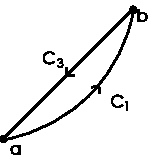
\includegraphics[width=0.3\textwidth]{figures/closedlineintegral.pdf}
		\caption{Closed line integral between $a$ and $b$ }
	\end{figure}
	
	Then
	
	$$
	\begin{aligned}
		\oint_C \mathbf{F} \cdot \mathrm{~d} \mathbf{r} & =\int_{C_1} \mathbf{F} \cdot \mathrm{~d} \mathbf{r}+\int_{C_3} \mathbf{F} \cdot \mathrm{~d} \mathbf{r} \\
		& =\left(\frac{e}{2}+\frac{1}{4}\right)-\frac{5}{3} \\
		& =-\frac{17}{12}+\frac{e}{2}
	\end{aligned}
	$$
\end{nex}

\section{Gradients and Differentials}

\begin{nthm}[*Line Integrals which depend on only endpoints]
	If $\mathbf{F}=\nabla f(\mathbf{r})$, then
	
	$$
	\int_C \mathbf{F} \cdot \mathrm{~d} \mathbf{r}=f(\mathbf{b})-f(\mathbf{a}),
	$$
	
	where $\mathbf{b}$ and $\mathbf{a}$ are the end points of the curve. Therefore the integral depends only on the end points and not the curve itself.
\end{nthm}

\begin{ndefi}[Conservative Vector Field]
	If $\mathbf{F}=\nabla f$ for some $f$, the $\mathbf{F}$ is called a conservative vector field.
\end{ndefi}

\begin{nrem}
	'Conservative' comes from mechanics where energy is conserved in a system. The work done around a closed curve is 0.
\end{nrem}

\begin{ndefi}[Exact Differential]
	A differential $\mathbf{F} \cdot \mathrm{d} \mathbf{r}$ is exact if there is an $f$ such that $\mathbf{F}=\nabla f$. Then
	
	$$
	\mathrm{d} f=\nabla f \cdot \mathrm{~d} \mathbf{r}=\frac{\partial f}{\partial x_i} \mathrm{~d} x_i .
	$$
\end{ndefi}

\begin{nprop}[Test for Conservative Vector Field]
	If $\mathbf{F}=\nabla f$ for some $f$, then
	
	$$
	\frac{\partial F_i}{\partial x_j}=\frac{\partial F_j}{\partial x_i}
	$$
	
	
	This is because both are equal to $\partial^2 f / \partial x_i \partial x_j$. For an exact differential, the result from the previous section reads
	
	$$
	\int_C \mathbf{F} \cdot \mathrm{~d} \mathbf{r}=\int_C \mathrm{~d} f=f(\mathbf{b})-f(\mathbf{a})
	$$
\end{nprop}

\begin{nprop}[Manipulations on differentials]
	
	$$
	\begin{aligned}
		\mathrm{d}(\lambda f+\mu g) & =\lambda \mathrm{d} f+\mu \mathrm{d} g \\
		\mathrm{~d}(f g) & =(\mathrm{d} f) g+f(\mathrm{~d} g)
	\end{aligned}
	$$
	
	Using these, it may be possible to find $f$ by inspection. We do this by integrating each component and seeing if they are equivalent. If they are, then the line integral is just this function evaluated between $\mathbf{a}$ and $\mathbf{b}$.
\end{nprop}

\section{Work and Potential Energy}

\begin{ndefi}[Work Done]
	If $\mathbf{F}(\mathbf{r})$ is a force, then $\int_C \mathbf{F} \cdot \mathrm{~d} \mathbf{r}$ is the work done by the force along the curve $C$. It is the limit of a sum of terms $\mathbf{F}(\mathbf{r}) \cdot \delta \mathbf{r}$, i.e. the force along the direction of $\delta \mathbf{r}$.
	
\end{ndefi}

\begin{ndefi}[Potential Energy]
	Given a conservative force $\mathbf{F}=-\nabla V, V(\mathbf{x})$ is the potential energy. Then
	
	$$
	\int_C \mathbf{F} \cdot \mathrm{~d} \mathbf{r}=V(\mathbf{a})-V(\mathbf{b}) .
	$$
	
	
	Therefore, for a conservative force, we have $\mathbf{F}=\nabla V$, where $V(\mathbf{r})$ is the potential energy.
\end{ndefi}

\section{Curvilinear Coordinates}

\begin{ndefi}[Curvilinear Coordinates]
	In a curvilinear coordinate system ( $u, v, w$ ), the coordinate lines - where two of the coordinates are constant and one varies - may be curved. These coordinate lines may be parametrised by the corresponding coordinate, so are given by $\boldsymbol{x}(u, v, w)$ with two of the coordinates fixed. The corresponding tangent vectors are therefore $\frac{\partial \boldsymbol{x}}{\partial u}, \frac{\partial \boldsymbol{x}}{\partial v}, \frac{\partial \boldsymbol{x}}{\partial w}$.
\end{ndefi}

\begin{ndefi}[Orthogonal and Scale Factors]
	The coordinate system is orthogonal if the three tangent vectors are mutually orthogonal at every point. We can then define an orthonormal basis $\left\{\boldsymbol{e}_u, \boldsymbol{e}_v, \boldsymbol{e}_w\right\}$ by normalising:
	
	$$
	\boldsymbol{e}_u=\frac{1}{h_u} \frac{\partial \boldsymbol{x}}{\partial u}, \quad \boldsymbol{e}_v=\frac{1}{h_v} \frac{\partial \boldsymbol{x}}{\partial v}, \quad \boldsymbol{e}_w=\frac{1}{h_w} \frac{\partial \boldsymbol{x}}{\partial w},
	$$
	
	where
	
	$$
	h_u=\left|\frac{\partial \boldsymbol{x}}{\partial u}\right|, \quad h_v=\left|\frac{\partial \boldsymbol{x}}{\partial v}\right|, \quad h_w=\left|\frac{\partial \boldsymbol{x}}{\partial w}\right|
	$$
	
	are called the scale factors.
\end{ndefi}

\begin{nrem}
	Geometrically, the scale factors tell you how much an infinitesimal region in $(u, v, w)$ coordinates is stretched at different points in real space. This is critical to account for during surface and volume integrals
\end{nrem}

\begin{nrem}
	It is relevant here to repeat the two coordinate basis from before:
	
	\begin{table}[H]
		\centering
		\renewcommand{\arraystretch}{1.6}
		\begin{tabular}{|p{0.45\textwidth}|p{0.45\textwidth}|}
			\hline
			\centering \textbf{Cylindrical polars} &
			\centering \textbf{Spherical polars} \tabularnewline
			\hline
			
			\multicolumn{2}{|c|}{\textbf{Conversion formulae}} \\
			\hline
			
			\[
			\begin{aligned}
				x_1 &= \rho \cos \varphi \\
				x_2 &= \rho \sin \varphi \\
				x_3 &= z
			\end{aligned}
			\]
			&
			\[
			\begin{aligned}
				x_1 &= r \sin \theta \cos \varphi \\
				x_2 &= r \sin \theta \sin \varphi \\
				x_3 &= r \cos \theta
			\end{aligned}
			\]
			\tabularnewline
			\hline
			
			\multicolumn{2}{|c|}{\textbf{Basis vectors}} \\
			\hline
			
			\[
			\begin{aligned}
				\mathbf e_\rho &= (\cos \varphi,\sin \varphi,0) \\
				\mathbf e_\varphi &= (-\sin \varphi,\cos \varphi,0) \\
				\mathbf e_z &= (0,0,1)
			\end{aligned}
			\]
			&
			\[
			\begin{aligned}
				\mathbf e_r &= (\sin \theta \cos \varphi,\sin \theta \sin \varphi,\cos \theta) \\
				\mathbf e_\varphi &= (-\sin \varphi,\cos \varphi,0) \\
				\mathbf e_\theta &= (\cos \theta \cos \varphi,\cos \theta \sin \varphi,-\sin \theta)
			\end{aligned}
			\]
			\tabularnewline
			\hline
		\end{tabular}
	\end{table}
	
\end{nrem}




\section{Differentiating Scalar Fields}

\begin{definition}[Gradient of a Scalar Field]
  The gradient of a scalar field $f: \mathbb{R}^3 \rightarrow \mathbb{R}$ is the operator

$$
\left.\nabla f\right|_{\boldsymbol{x}}=\lim _{\mathrm{d}(S) \rightarrow 0} \frac{1}{|V|} \oint_S f \hat{\boldsymbol{n}} d S,
$$

where $S$ is a closed surface around $\boldsymbol{x}$ with outward normal $\hat{\boldsymbol{n}}$, enclosed volume $|V|$, and diameter $\mathrm{d}(S)=\sup _{\boldsymbol{x}, \boldsymbol{y} \in S}|\boldsymbol{x}-\boldsymbol{y}|$.
\end{definition}

\begin{rem}
  We note that $\nabla f$ is a vector field $\mathbb{R}^3 \rightarrow \mathbb{R}^3$ and our intuition is that it points in the direction of the fastest increase of $f$. 
\end{rem}

\begin{proposition}
  In Cartesian coordinates,

$$
\boldsymbol{\nabla} f=\frac{\partial f}{\partial x} \boldsymbol{e}_1+\frac{\partial f}{\partial y} \boldsymbol{e}_2+\frac{\partial f}{\partial z} \boldsymbol{e}_3 .
$$
\end{proposition}

\noindent This tells us that $\nabla f$ is a differential operator, acting on a scalar field and returning a vector field. We see a similar formula from Calculus I but the integral we have defined here should work independent of any particular choice of coordinates. To prove our proposition we use the following lemma:

\begin{lemma}[Mean Value Theorem for Double Integrals]
  If a scalar field $f: \mathbb{R}^2 \rightarrow \mathbb{R}$ is continuous on a closed, bounded and connected domain $A \subset \mathbb{R}^2$ then there exists $\boldsymbol{x}_* \in A$ such that

$$
\int_A f d S=|A| f\left(\boldsymbol{x}_*\right)
$$
\end{lemma}

\noindent This formula is analagous for the 1-d result of mean value theorem depicted in the figure below. In 1-d we have that if $f(x)$ is continuous on $[a,b]$ then there exists $x_* \in [a,b]$ such that $\int_a^b f(x) d x=(b-a) f\left(x_*\right)$ .


\begin{figure}[H]
  \centering
  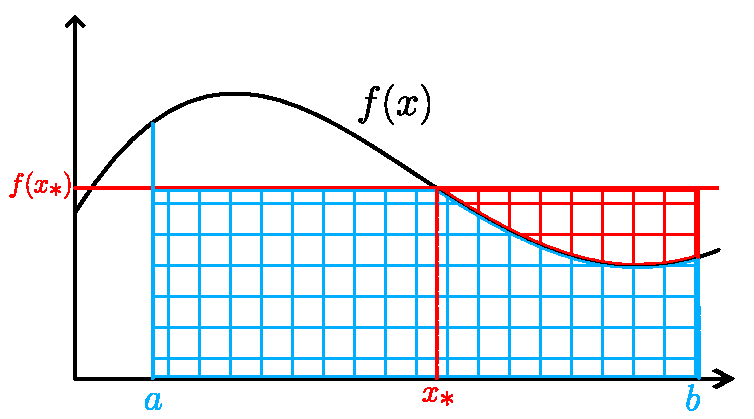
\includegraphics[width=0.67\textwidth]{figures/mthmchp3im1}
  \caption{1D representation of Mean Value Theorem}
  \label{fig:Mean Value 2D}
\end{figure}

\noindent Lemma 3.1.4 says that there is some particular point $\boldsymbol{x}_*$ where $f$ attains its average value, $f\left(x_*\right)=\frac{1}{|A|} \int_A f d S$.

%proof goes here%

\begin{proposition}
  In orthogonal curvilinear coordinates $(u, v, w)$, the gradient has the expression

$$
\boldsymbol{\nabla} f=\frac{1}{h_u} \frac{\partial f}{\partial u} \boldsymbol{e}_u+\frac{1}{h_v} \frac{\partial f}{\partial v} \boldsymbol{e}_v+\frac{1}{h_w} \frac{\partial f}{\partial w} \boldsymbol{e}_w .
$$
\end{proposition}

\begin{example}[Computing $\nabla z$ in both Cartesian and Spherical Coordinates]

In Cartesians, we have

$$
\boldsymbol{\nabla}(z)=\frac{\partial z}{\partial x} \boldsymbol{e}_1+\frac{\partial z}{\partial y} \boldsymbol{e}_2+\frac{\partial z}{\partial z} \boldsymbol{e}_3=\boldsymbol{e}_3 .
$$

\noindent In spherical coordinates $(r, \theta, \phi)$, recall that $z=r \cos \theta$. So Proposition 3.2 gives

$$
\begin{aligned}
\boldsymbol{\nabla}(r \cos \theta) & =\frac{1}{h_r} \frac{\partial}{\partial r}(r \cos \theta) \boldsymbol{e}_r+\frac{1}{h_\theta} \frac{\partial}{\partial \theta}(r \cos \theta) \boldsymbol{e}_\theta+\frac{1}{h_\phi} \frac{\partial}{\partial \phi}(r \cos \theta) \boldsymbol{e}_\phi \\
& =\frac{\partial}{\partial r}(r \cos \theta) \boldsymbol{e}_r+\frac{1}{r} \frac{\partial}{\partial \theta}(r \cos \theta) \boldsymbol{e}_\theta \\
& =\cos \theta \boldsymbol{e}_r-\sin \theta \boldsymbol{e}_\theta .
\end{aligned}
$$

\noindent We recognise this as $\boldsymbol{e}_3$ again.

\end{example}

\begin{remark}
Observe that our coordinate formula, and hence $\boldsymbol{\nabla} f$, extends to scalar fields on any $\mathbb{R}^n$, and giving always a vector in $\mathbb{R}^n$. Very high-dimensional vectors are commonly used in machine learning algorithms.
\end{remark}

\section{Differentiating Vector Fields}

There are two standard ways to differentiate a vector field $\mathbf{f} : \mathbb{R}^3 \rightarrow \mathbb{R}^3$:

\begin{itemize}
  \item The divergence of $\boldsymbol{f}$ is the scalar field

$$
\left.\boldsymbol{\nabla} \cdot \boldsymbol{f}\right|_{\boldsymbol{x}}=\lim _{\mathrm{d}(S) \rightarrow 0} \frac{1}{|V|} \oint_S \hat{\boldsymbol{n}} \cdot \boldsymbol{f} d S .
$$

\item The curl of $\boldsymbol{f}$ is the vector field

$$
\boldsymbol{\nabla} \times\left.\boldsymbol{f}\right|_{\boldsymbol{x}}=\lim _{\mathrm{d}(S) \rightarrow 0} \frac{1}{|V|} \oint_S \hat{\boldsymbol{n}} \times \boldsymbol{f} d S .
$$
\end{itemize}

\begin{blackbox}[Vector Fields]
  This is an example of a black bix
\end{blackbox} 


